\documentclass[a4paper]{article}

%% Language and font encodings
\usepackage[english]{babel}
\usepackage[utf8x]{inputenc}
\usepackage[T1]{fontenc}

%% Sets page size and margins
\usepackage[a4paper,top=3cm,bottom=2cm,left=3cm,right=3cm,marginparwidth=1.75cm]{geometry}

%% Useful packages
\usepackage{amsmath}
\usepackage{graphicx}
\usepackage[colorinlistoftodos]{todonotes}
\usepackage[colorlinks=true, allcolors=blue]{hyperref}

\title{Reporte de Actividad 8}
\author{Valenzuela Terán Jonás}

\begin{document}
\maketitle

\section{Introducción}

La actividad es similar a las anteriores, pero difiere en que utiliza un modelo diferente, además de gráficas que poseen un campo vectorial, esto es con el objetivo de poder aplicar lo que aprendimos a otro contexto, y a familiarizarnos más con modelos no lineales y caóticos, que la mayor parte del tiempo se presentan en la naturaleza y en la física.

Utilizamos las mismas herramientas, estas son jupyter lab, con lenguaje de programación python y librerías importadas para graficación, cálculos y soluciones numéricas. La ventaja de esto es la gran comunidad que soporta estas herramientas, que nos permite encontrar soluciones si algo no termina bien.


\section{Modelo de Van der Pol}

Es un oscilador no conservativo con amortiguamiento no lineal, fue propuesto por el ingeniero electrico Balthasar van der Pol en el trabajo, encontro que existen oscilaciones estables, que ahora conocemos como ciclo límite, y los movimientos tienden a el.

\begin{center}
	$\displaystyle \frac{d^2 x}{d t^2} - \mu (1 - x^2) \frac{dx}{dt} + x = 0$
\end{center}

Donde $x$ es la posición, que es función del tiempo, y $\mu$ es un parámetro que indica la no linealidad y el amortiguamiento.


\section{Exploración de las soluciones del modelo en el Espacio Fase}

Se replicaron las gráficas mostradas en el articulo de Van der Pol, definiendo el modelo y los parámetros, para obtener la gráfica de los datos obtenidos, se pudo observar que el factor de no linealidad influye mucho en el resultado, además, que todas las diferentes condiciones iniciales, terminan convergiendo al ciclo límite en el plano de fase (velocidad contra posición).

Se intentó adaptar el campo vectorial al modelo, para ver claramente como diferentes posiciones tienden a el ciclo límite con diferente fuerza, y en el camino se observó como actúan las flechas de campo vectorial con diferentes modelos.


\section{Resultados y discusión}

Ya en el entorno de programación, introduciendo el modelo y los parámetros necesarios, se obtuvieron las siguientes gráficas:

\begin{center}
	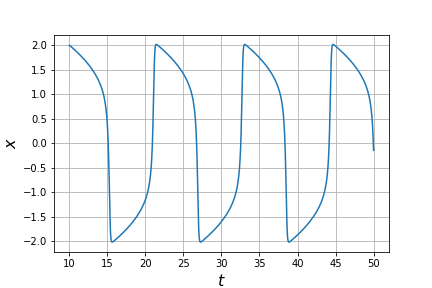
\includegraphics[height=5cm]{xtsinf.png}
\end{center}

Se pudo obtener una gráfica similar a la del articulo, de posición contra tiempo, analizando el movimiento, encontramos que es periódico, esta se refiere a una \textit{oscilación relajante}, este movimiento es al que se tiende después de un tiempo.

\begin{center}
	$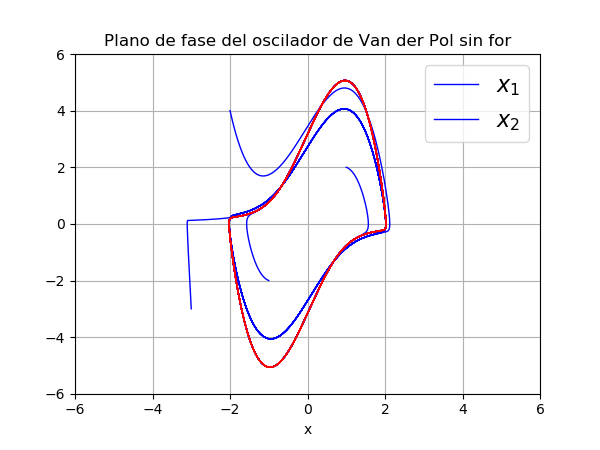
\includegraphics[height=5cm]{fase.png}$
\end{center}

La tercera figura nos muestra como, con el mismo coeficiente de no linealidad, y con diferentes condiciones iniciales de posición y velocidad, el movimiento tiende al mismo (rojo), el ciclo límite, a esta figura se le conoce como el plano de fase.

\begin{center}
	$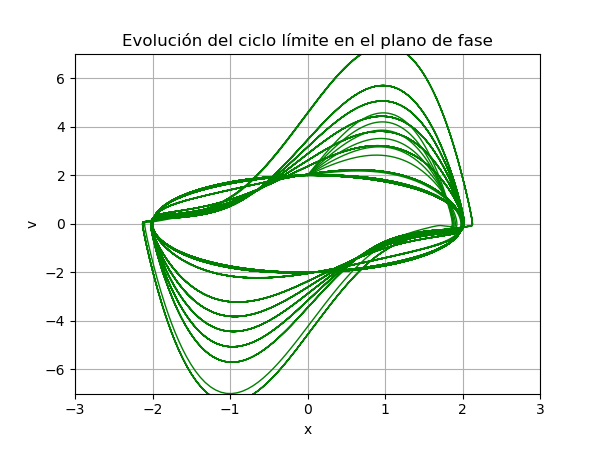
\includegraphics[height=5cm]{evolucion.png}$
\end{center}

Ahora vemos como al cambiar el coeficiente de no linealidad, y manteniendo fijas las condiciones iniciales, cambia el ciclo límite, asemejando una circunferencia al acercarse a 0, y deformándose al crecer.

\begin{center}
	$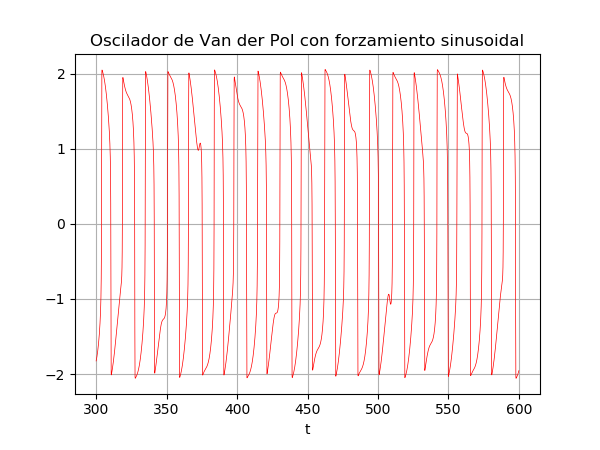
\includegraphics[height=5cm]{xtconf.png}$
\end{center}

Finalmente, agregamos forzamiento sinusoidal al modelo, y encontramos que también tiende a un movimiento periódico, pero de una mayor complejidad.


\section{Conclusiones del estudio}

Pudimos observar otro modelo, y más ejemplos de no linealidad con la misma herramienta, adaptando esta a lo que queremos representar y además, exploramos la representación de campos vectoriales para estos modelos, esto también comprueba la eficiencia y confiabilidad de los métodos numéricos utilizados para modelar, ya que describen correctamente los datos con buena precisión y mantienen periodicidad.

\section{Bibliografía}

\begin{itemize}
\item (2018). Van der Pol oscillator. 10 de abril 2018, de Wikipedia Sitio web:

\textit{https://en.wikipedia.org/wiki/Van\_der\_Pol\_oscillator}


\item Takashi Kanamaru. (2007). Van der Pol oscillator. 10 de abril 2018, de Scholarpedia Sitio web:
\textit{http://www.scholarpedia.org/article/Van\_der\_Pol\_oscillator}


\item Various authors. (2015). Matplotlib: lotka volterra tutorial. 10 de abril 2018, de SciPy Cookbook Sitio web:
\textit{http://scipy-cookbook.readthedocs.io/items/LoktaVolterraTutorial.html}


\item N.Kh. Rozov. (2011). Van der Pol equation. 12 de abril 2018, de Encyclopedia of Mathematics Sitio web:
\textit{https://www.encyclopediaofmath.org/index.php/Van\_der\_Pol\_equation}
\end{itemize}



\section{Apéndice}

\begin{itemize}
\item     Este ejercicio pareciera similar al desarrollado en las actividades 6 y 7. ¿Qué aprendiste nuevo?

Aprendí sobre la representación de campos vectoriales, y nuevas formas de definir el modelo en el entorno de programación, esto crea muchas maneras de lograr el mismo objetivo, todas útiles y eficientes.

\item     ¿Qué fue lo que más te llamó la atención del oscilador de Van der Pol?

Que mantiene la misma figura el ciclo límite, sin importar las condiciones iniciales, y que se puede obtener información valiosa analizando el plano de fase.

\item     Has escuchado ya hablar de caos. ¿Por qué sería importante estudiar este oscilador?

Porque tiene utilidad en algunas áreas de la ciencia, y es un ejemplo de un modelo caótico que se presenta en la naturaleza.

\item     ¿Qué mejorarías en esta actividad?

Fue interesante, y buena dinámica que la representación del campo vectorial fuera un reto, y el ejemplo proporcionado aseguró que fuera un reto ya que son contextos muy distintos, pero se apreciara si existiera mayor explicación sobre como funciona la manera en que definen el modelo.

\item     ¿Algún comentario adicional antes de dejar de trabajar en Jupyter con Python?

Siento que no vimos a detalle como funcionan los ciclos y los arreglos en python, pero como tenemos esas bases de fortran, tengo entendido que será fácil extenderlo a python con suficiente investigación.

\item     Cerramos la parte de trabajo con Python ¿Que te ha parecido?

Me parece muy bien, la herramienta es muy útil y de multiples usos, me gustaría conocer otro tipo de aplicaciones que puede ofrecer esta herramienta.
\end{itemize}




\end{document}